\documentclass{sigchi}

% Use this command to override the default ACM copyright statement
% (e.g. for preprints).  Consult the conference website for the
% camera-ready copyright statement.

%% EXAMPLE BEGIN -- HOW TO OVERRIDE THE DEFAULT COPYRIGHT STRIP -- (July 22, 2013 - Paul Baumann)
% \toappear{Permission to make digital or hard copies of all or part of this work for personal or classroom use is      granted without fee provided that copies are not made or distributed for profit or commercial advantage and that copies bear this notice and the full citation on the first page. Copyrights for components of this work owned by others than ACM must be honored. Abstracting with credit is permitted. To copy otherwise, or republish, to post on servers or to redistribute to lists, requires prior specific permission and/or a fee. Request permissions from permissions@acm.org. \\
% {\emph{CHI'14}}, April 26--May 1, 2014, Toronto, Canada. \\
% Copyright \copyright~2014 ACM ISBN/14/04...\$15.00. \\
% DOI string from ACM form confirmation}
%% EXAMPLE END -- HOW TO OVERRIDE THE DEFAULT COPYRIGHT STRIP -- (July 22, 2013 - Paul Baumann)

% Arabic page numbers for submission.  Remove this line to eliminate
% page numbers for the camera ready copy
% \pagenumbering{arabic}

% Load basic packages
\usepackage{balance}  % to better equalize the last page
\usepackage{graphics} % for EPS, load graphicx instead 
\usepackage[T1]{fontenc}
\usepackage{txfonts}
\usepackage{mathptmx}
\usepackage[pdftex]{hyperref}
\usepackage{color}
\usepackage{booktabs}
\usepackage{textcomp}
% Some optional stuff you might like/need.
\usepackage{microtype} % Improved Tracking and Kerning
% \usepackage[all]{hypcap}  % Fixes bug in hyperref caption linking
\usepackage{ccicons}  % Cite your images correctly!
% \usepackage[utf8]{inputenc} % for a UTF8 editor only

% If you want to use todo notes, marginpars etc. during creation of your draft document, you
% have to enable the "chi_draft" option for the document class. To do this, change the very first
% line to: "\documentclass[chi_draft]{sigchi}". You can then place todo notes by using the "\todo{...}"
% command. Make sure to disable the draft option again before submitting your final document.
\usepackage{todonotes}

% Paper metadata (use plain text, for PDF inclusion and later
% re-using, if desired).  Use \emtpyauthor when submitting for review
% so you remain anonymous.
\def\plaintitle{Good Vibrations}
\def\plainauthor{First Author, Second Author, Third Author,
  Fourth Author, Fifth Author, Sixth Author}
\def\emptyauthor{}
\def\plainkeywords{Authors' choice; of terms; separated; by
  semicolons; include commas, within terms only; required.}
\def\plaingeneralterms{Documentation, Standardization}

% llt: Define a global style for URLs, rather that the default one
\makeatletter
\def\url@leostyle{%
  \@ifundefined{selectfont}{
    \def\UrlFont{\sf}
  }{
    \def\UrlFont{\small\bf\ttfamily}
  }}
\makeatother
\urlstyle{leo}

% To make various LaTeX processors do the right thing with page size.
\def\pprw{8.5in}
\def\pprh{11in}
\special{papersize=\pprw,\pprh}
\setlength{\paperwidth}{\pprw}
\setlength{\paperheight}{\pprh}
\setlength{\pdfpagewidth}{\pprw}
\setlength{\pdfpageheight}{\pprh}

% Make sure hyperref comes last of your loaded packages, to give it a
% fighting chance of not being over-written, since its job is to
% redefine many LaTeX commands.
\definecolor{linkColor}{RGB}{6,125,233}
\hypersetup{%
  pdftitle={\plaintitle},
% Use \plainauthor for final version.
%  pdfauthor={\plainauthor},
  pdfauthor={\emptyauthor},
  pdfkeywords={\plainkeywords},
  bookmarksnumbered,
  pdfstartview={FitH},
  colorlinks,
  citecolor=black,
  filecolor=black,
  linkcolor=black,
  urlcolor=linkColor,
  breaklinks=true,
}

% create a shortcut to typeset table headings
% \newcommand\tabhead[1]{\small\textbf{#1}}

% End of preamble. Here it comes the document.
\begin{document}

\title{\plaintitle}

\numberofauthors{5}
\author{%
  \alignauthor{Alisa Ananjeva\\
    \affaddr{Aalborg University}\\
    \affaddr{Selma Lagerl{\"o}fs Vej 300
DK-9220 Aalborg East}\\
    \email{ananj14@student.aau.dk}}\\
  \alignauthor{Jesper Quist Jensen\\
    \affaddr{Aalborg University}\\
    \affaddr{Selma Lagerl{\"o}fs Vej 300
DK-9220 Aalborg East}\\
    \email{jqje14@student.aau.dk}}\\
  \alignauthor{Kenneth Uldbjerg J{\o}rgensen\\
    \affaddr{Aalborg University}\\
    \affaddr{Selma Lagerl{\"o}fs Vej 300
DK-9220 Aalborg East}\\
    \email{kuja11@student.aau.dk}}\\
  \alignauthor{Rasmus Thygesen Larsen\\
    \affaddr{Aalborg University}\\
    \affaddr{Selma Lagerl{\"o}fs Vej 300
DK-9220 Aalborg East}\\
    \email{rlarse14@student.aau.dk}}\\
  \alignauthor{Simon Boel Poulsen\\
    \affaddr{Aalborg University}\\
    \affaddr{Selma Lagerl{\"o}fs Vej 300
DK-9220 Aalborg East}\\
    \email{sbpo14@student.aau.dk}}\\
}

\maketitle

\begin{abstract}
In this study we show that it is possible to design and develop a calm wearable navigation system for cyclists, based only on vibro-tactile output. Our design relies on vibro-tactile tactons utilised to communicate navigation instructions. Through several design iterations, and user tests the development of an understandable interaction is documented. We found that users were able to easily comprehend tactons and associate them with navigational instructions, when communicated in a relevant context. We also found that it is important to keep the user sufficiently informed at all times, to avoid loss of trust in system - however overly informing the user can also lead to confusion.
\end{abstract}

\category{H.5.m.}{Information Interfaces and Presentation
  (e.g. HCI)}{Miscellaneous}

\keywords{Vibro-tactile modality; Navigation; Vibration; alternative interaction; Cycling navigation; Attention; Calm Technology; Periphery; Wearable, Bicycle}

\section{Introduction}
Cycling is an activity which is very attention demanding, therefore ways of interacting with technology while cycling are challenging. Cyclist often have a need of directions, for which smartphones provide ideal navigation applications. However traditional ways of interacting with smartphones are far from ideal for cyclists. Since it requires the user to either continuously stop cycling to look at their phone, or perform potentially dangerous multitasking interaction, by taking one hand of the handlebar and taking attention away from traffic to look at the screen. 
\newline
\newline
Some navigation applications solve this by using audio output for interacting, however this also proposes some challenges, since audio instructions can potentially be hard to hear and perceive, in a high stress traffic situation. Additionally using audio disengages the user from the surroundings and traffic, by blocking the audio modality.
\subsection{Calm Technology}
In order to let the user keep attention on the surroundings, an \textit{unobtrusive interaction} is required. In order to obtain this, the eight principles of calm technology, described by Amber Case, can be utilised \cite{case15}. The principles  defines how to make a technical system that demands the minimum amount of attention from the user, by only interacting with the user when necessary and choosing the right form of  interaction.  
\newline
\newline 
While developing the system, it was chosen to base the interaction on vibration as output technology, since this complies well with calm technology principles about technology making use of the periphery, and communicating without speaking.
\section{Related Work}
There are several studies made regarding vibro-tactile interaction, especially how the vibration can be perceived. 
\newline
Brown et al. defines a term \textit{''tacton''}, and introduced five parameters, which influence the physical vibro-tactile output \cite{brown06}. These five parameters are:
\begin{itemize}
\item \textbf{Rhythm}: a group of several pulses, with different durations and gaps between them.
\item \textbf{Frequency}: waves of a vibration.
\item \textbf{Intensity}: vibration amplitude.
\item \textbf{Roughness}: combination of different frequencies and intensities make roughness-
\item \textbf{Spatial location}: the placement of a vibration module.
\end{itemize}
These parameters are important while exploring how the vibro-tactile interaction can be made, and how different parameters affect the perception of the interaction. When combining these parameters, distinguishable tactons can be created, that ensure more efficient vibro-tactile interaction. Regarding the distinguishability, Lee and Starner conducted a study where people's ability to distinguish 24 different tactons was tested. It was found that after limited training, participants were better at distinguishing between the tactons \cite{lee10}. Which shows that not only the five parameters introduced by Brown et al. can aid distinguishability, but there is also a learning curve to be expected. 
\newline
\newline
Some parameters seems to affect peoples' ability to distinguish between tactons, such as Intensity and spatial location. Intensity was harder to distinguish between compared to spatial location, which was easy distinguishable. 
\newline
\newline
There are other phenomena that can affect vibro-tactile interaction, and how people perceive it \cite{myles07}: 
\begin{itemize}
\item \textbf{Masking}: occurs when there are multiple vibration stimuli on the same time and space. Making it hard to understand the tacton. 
\item \textbf{Adaption}: occurs when one tacton is given constantly, making it appear weaker over time.
\end{itemize}
One of the main concerns while developing a calm technology that utilises vibro-tactile interaction is whether users can perceive the vibration without it being obtrusive. Pielot and de Oliveira evaluated whether vibration could stay in people's periphery, thus being unobtrusive. They found that when vibration is just above the threshold people would be aware of the vibration but would not deal a great deal of attention to it. Thus proving this stimulation useful for non-obtrusive communication, even though they perceived the vibration \cite{pielot13}.  
\newline
\newline
There are different implementations of vibro-tactile modality as an information channel. Heuten et al. created a vibro-tactile wayfinding system, by putting vibration modules in a belt which could then communicate the way to go \cite{heuten08}. Their findings showed that people can navigate using vibro-tactile modality, indicating that people can understand the information transferred through tactons. 
Bial et al. used vibration to inform cyclists of their optimal pedalling frequency, by placing vibration modules in cyclists shoes \cite{bial11}. This study supports the finding from Heuten et al., regarding people's ability to understand vibro-tactile modality. In addition to that, Bial et al. found that users experienced vibration as a fun alternative way of getting instructions. 
\newline
\newline
Popinga et al., researched the application of vibro-tactile interaction as a navigational tool, in addition to a visual display showing a map on tourists bicycles. They found that it is possible to use vibro-tactile modality to navigate on a bicycle \cite{poppinga09}.
\newline
\newline
These articles show other researchers' approach towards vibro-tactile modality, how it is perceived by users and how it can be implemented in many different ways. Showing that even though vibro-tactile modality has its constraints, it can be used as alternative to conventional navigation, which uses audio and visual modality.

\section{Design Process}
In our study we followed Buxtons method for designing a product, which revolves around an iterative design process, where ideas are iteratively added and evolved, in what Buxton describes as \textit{Concepts Generation} \cite{buxton07}. The designs are then reviewed or tested, to gain insight for improvement and eliminate some ideas, in what Buxton describes as \textit{Controlled Convergence}. The process is a funnel approach, as shown in figure \ref{fig:1_development_model}, where the design starts wide, and then narrows in on a final concept.
\begin{figure}
\centering
  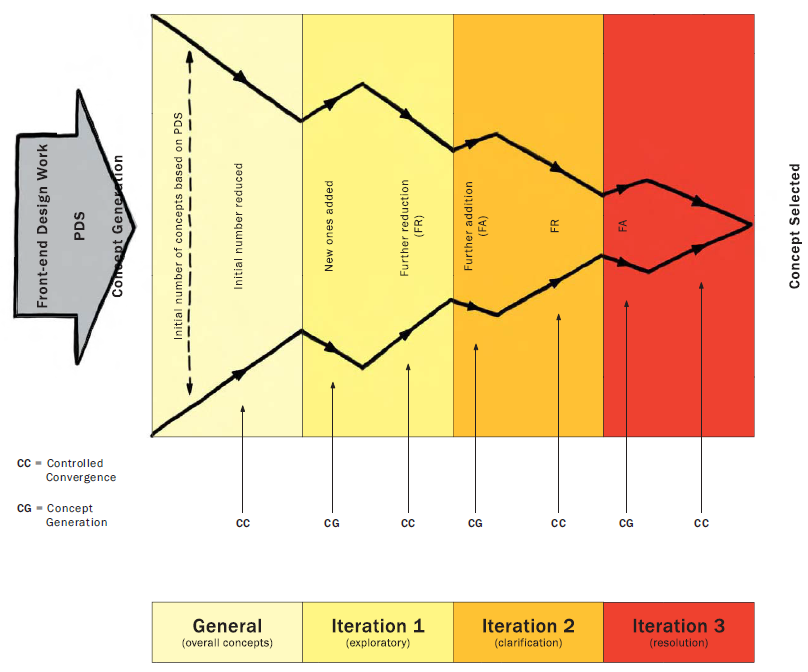
\includegraphics[width=1.02\columnwidth]{figures/1_development_model.png}
  \caption{Bill Buxton's development model.
}\label{fig:1_development_model}
\end{figure}
In our approach we start with a wide concepts generation, and then moved to user-based tests, first as a qualitative lab based test for exploring different prototype concepts, and later as a field evaluation with a bulky but functional prototype. We then improved the design to small Bluetooth connected vibrational wristbands, created a fully functional smartphone companion application and created and tested additional tactons for the system. A final user based field evaluation was performed, where the wearable wristbands with functioning hardware was equipped on the participants for evaluation.
\newline
\newline
Prior to the initial design, some requirement specifications which contained some general aspects that the final design concept should aim to fulfil was followed. In the initial design phase we aimed to generate as many ideas as possible for designing calm interaction for bicycle navigation. Most ideas were created initially through stages of sketching, and reviewed by a discussion. Additionally paper prototypes, example seen in figure \ref{fig:handle-button}, were created of different designs, to visualise how ideas would work.
\begin{figure}
\centering
  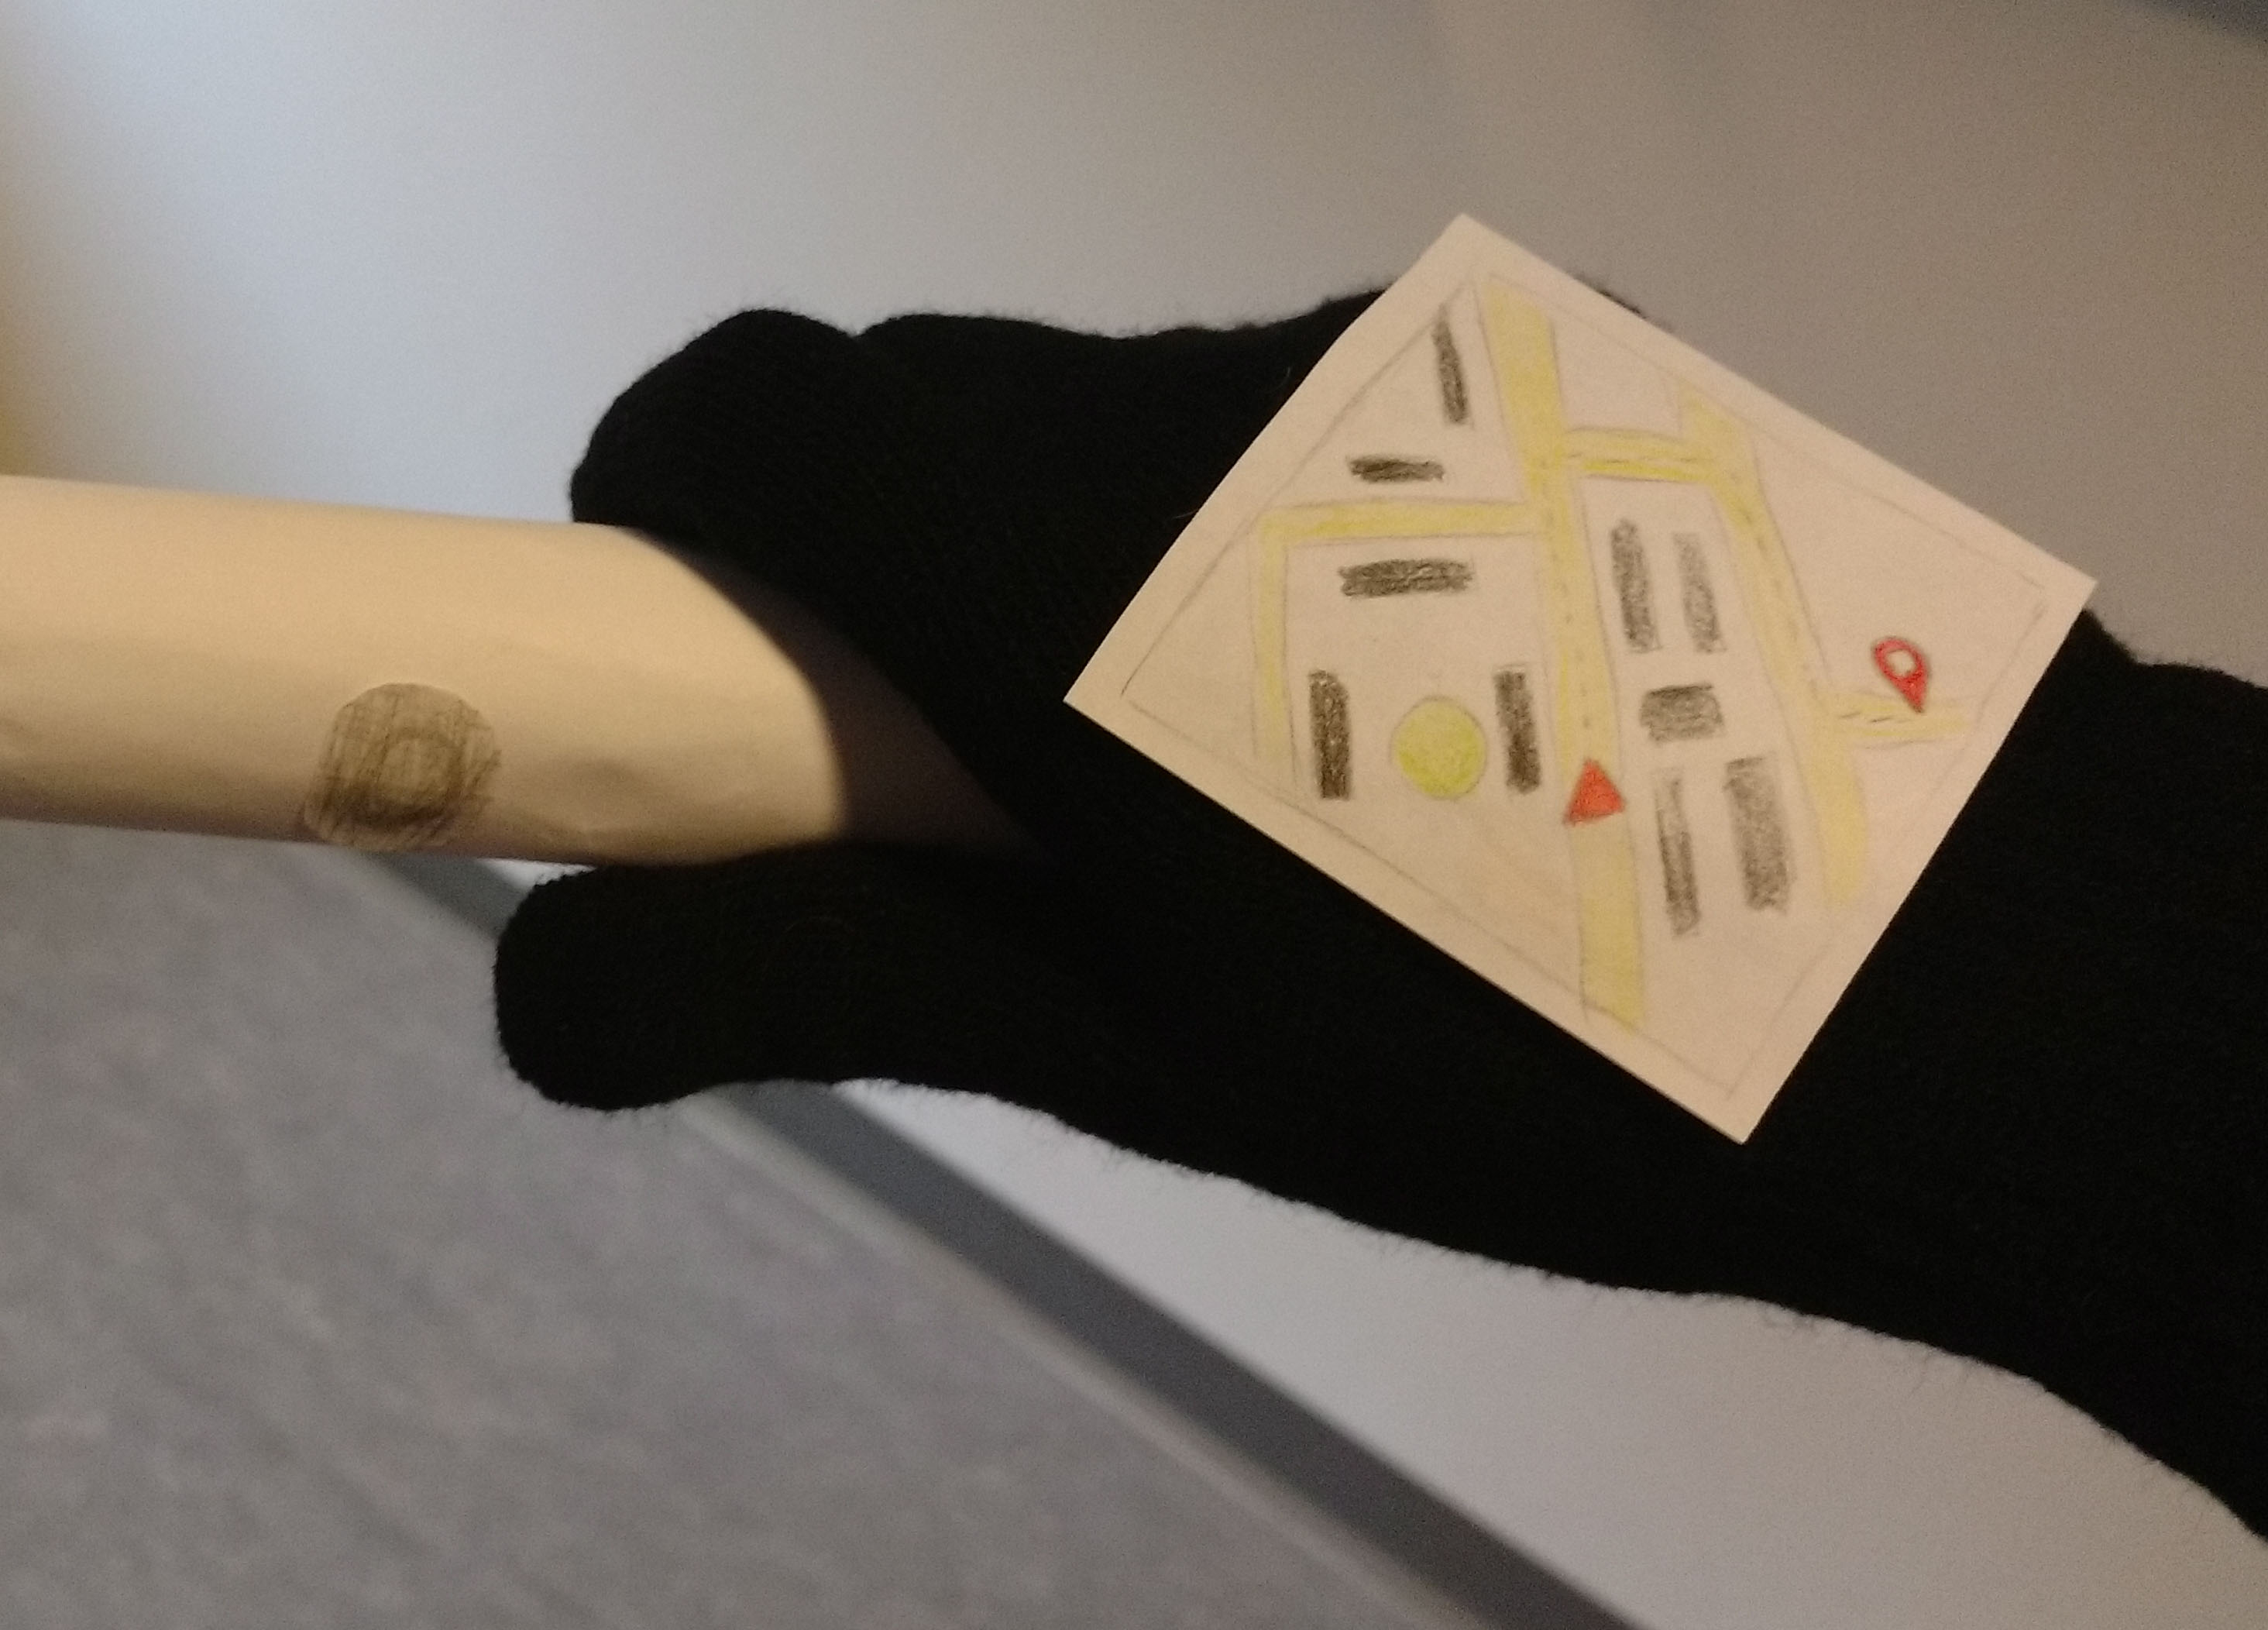
\includegraphics[width=0.8\columnwidth]{figures/handle-button.jpg}
  \caption{An example of the paper prototypes created during initial design.}\label{fig:handle-button}
\end{figure}
After the initial design process some potential ideas were chosen to be tested, these were: a vibration output through a helmet, vibration output in a pair of gloves and visual output on the handlebars. . Every concept had the objective to inform the user of turns on their route, by vibrating/blinking when the user has to turn.
\section{First Lab test: Exploratory}
In an initial qualitative exploratory prototype lab test, the three different design concepts were tested on four participants. For each design idea a prototype was created, using littleBits, which allow building simple functioning prototypes. The participants were asked to cycle on a stationary bicycle while watching a point-of-view video of a cycling route to mimic the cycling experience as much as possible. The setup is shown in figure \ref{fig:eval1_setup}. The user then received signals for navigational instructions in synchronisation with turns occurring on video. This was done through a wizard-of-oz type setup, with a moderator managing the output being send to the test participant. An additional test conductor was present to guide the test participants, and to note observations during the test. Each prototype was tested sequentially, in a random order, followed by a short semi-structured interview, and a final interview after testing all prototypes.
\begin{figure}[!b]
\centering
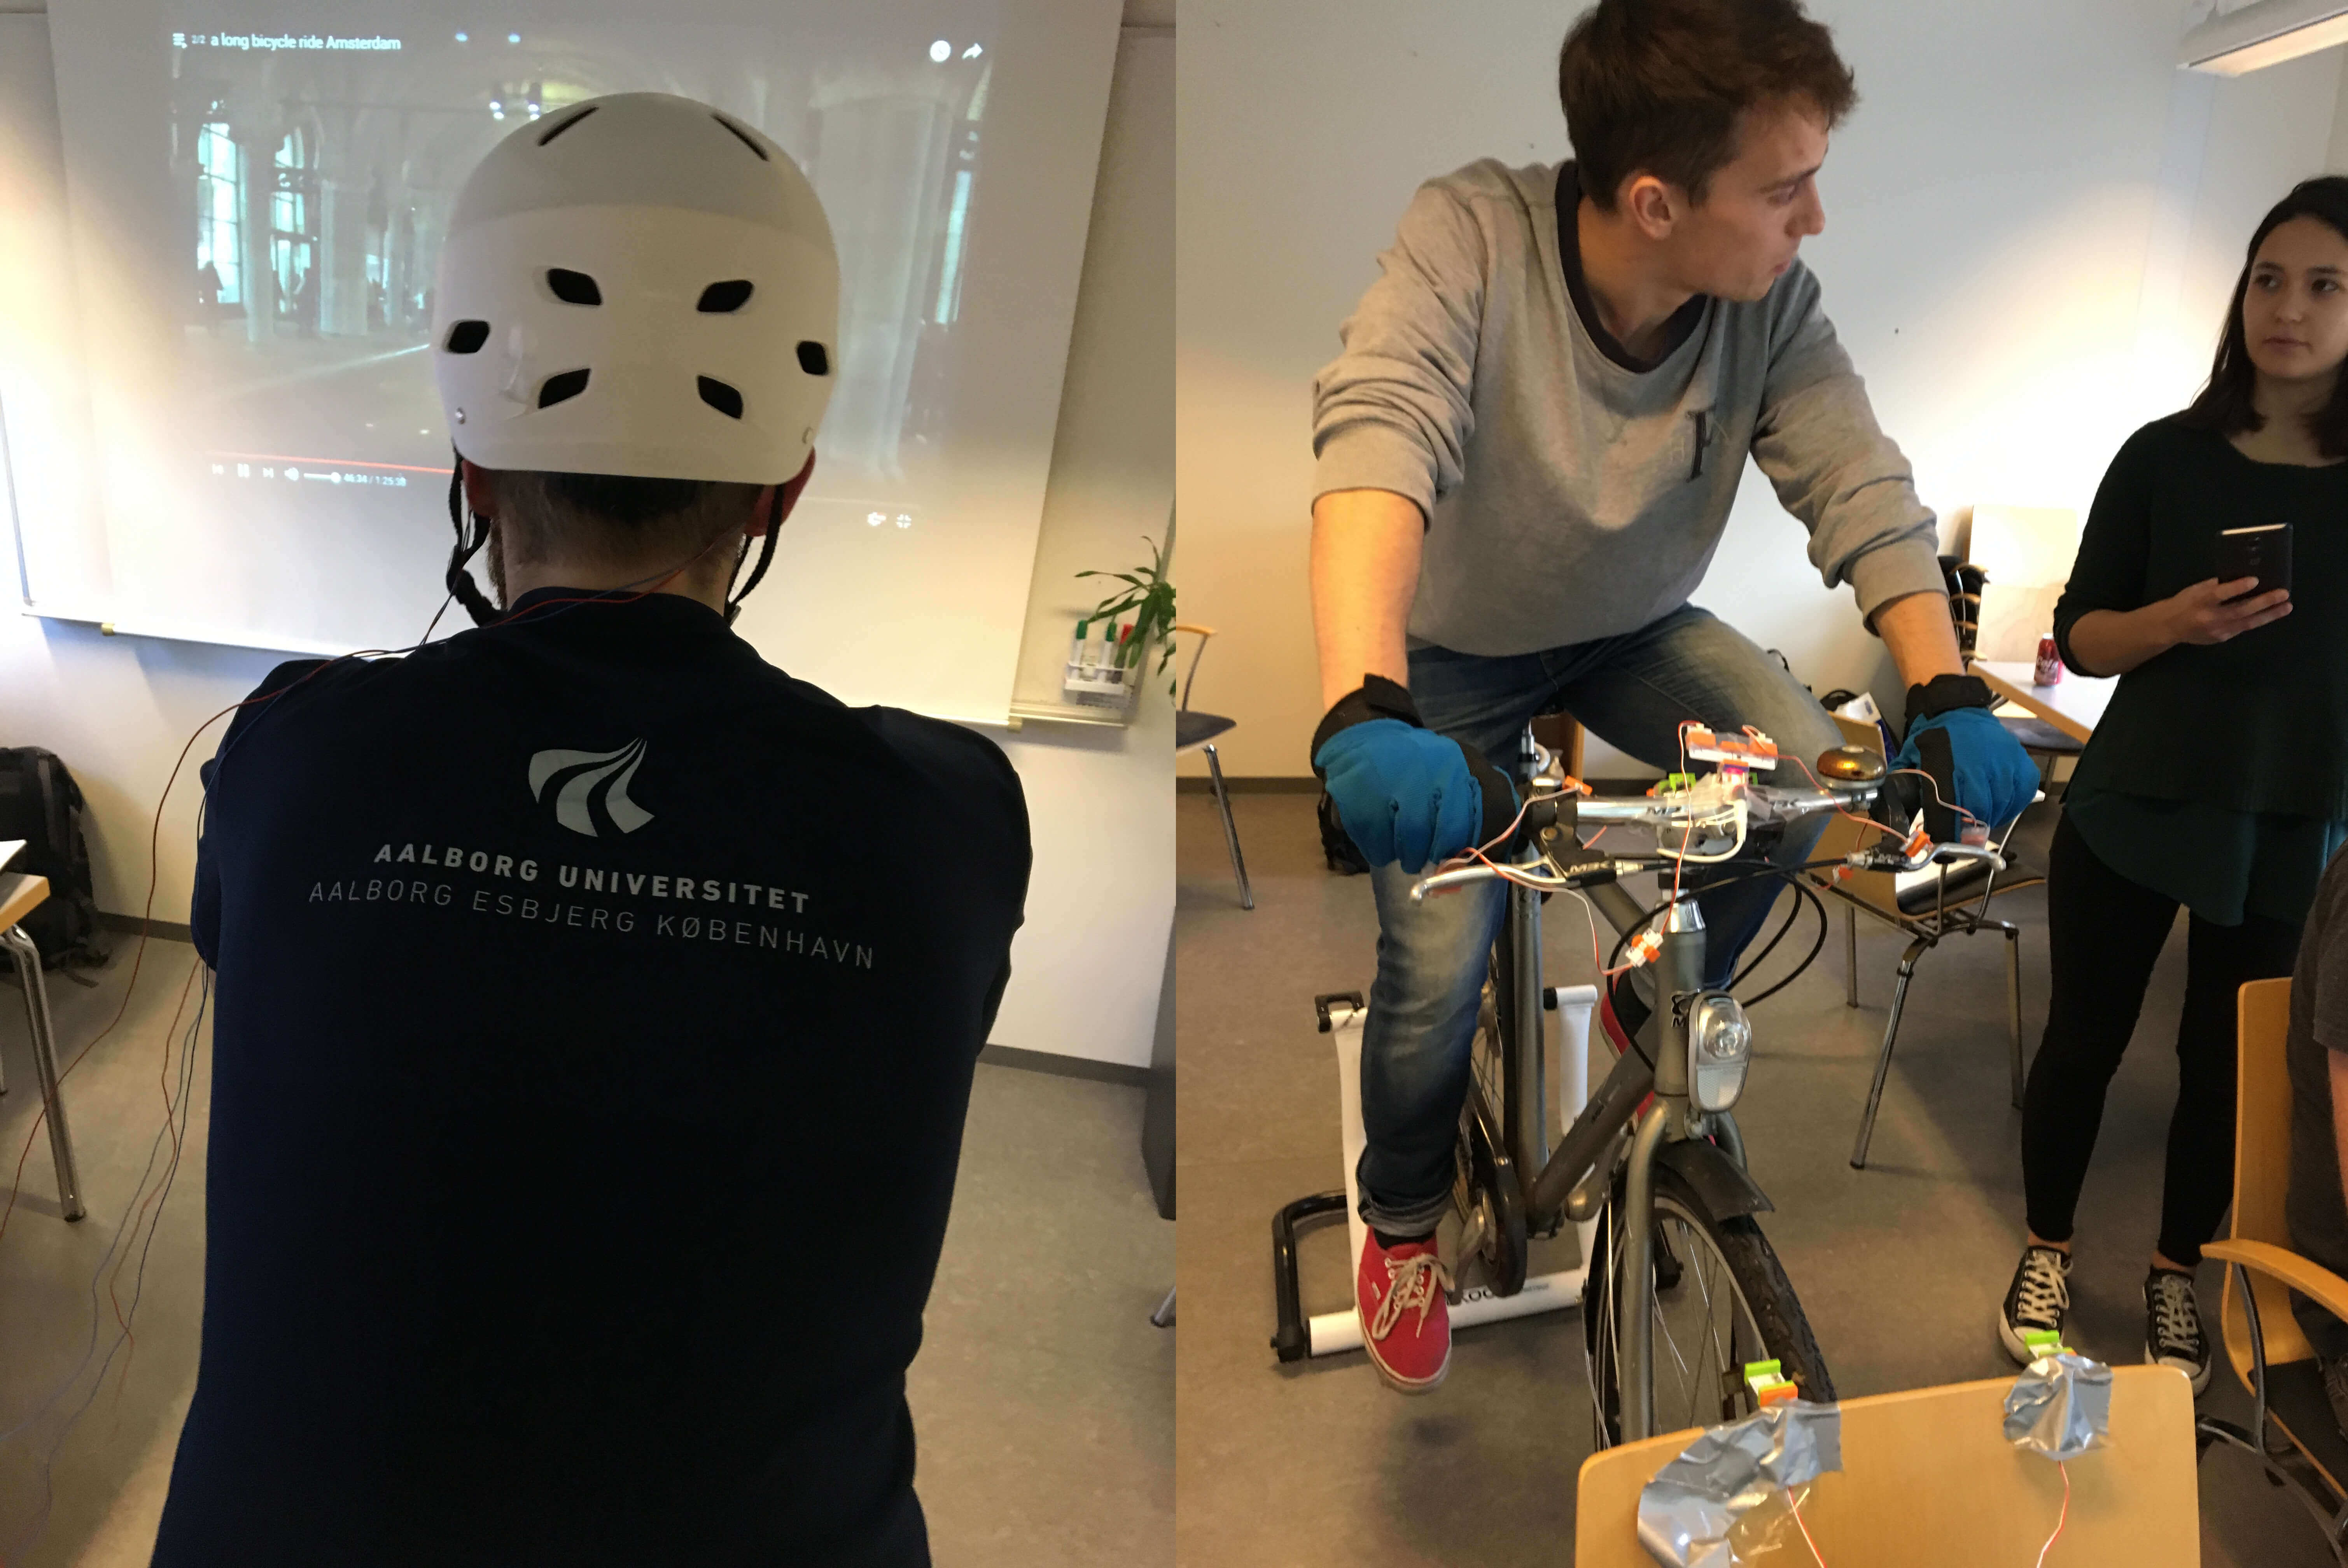
\includegraphics[width=0.9\columnwidth]{figures/eval1_setup.jpg}
\caption{Depiction of the lab test setting.}
\label{fig:eval1_setup}
\end{figure}
The results from the test showed that participants preferred vibration to light output, since light required them to look away from the video screen which was impractical, and potentially safety critical. Vibration was found to be simple to understand and unobtrusive. The vibrational helmet was found to be impractical, since some users could not feel the vibration, due to the helmet size not fitting completely, while some also mentioned the vibration as being uncomfortable. The gloves were preferred by most participants, however it was noted that they would not be practical in a warm environment.
\section{First Field Test: Prove of Concept}
Based on the findings from the exploratory Labtest, a functioning prototype was created for a field evaluation. It had gloves, one for each hand, with vibration modules, these were connected to an Arduino Uno. The system can be seen in figure \ref{fig:enitial_prototype}. Additionally a mobile application was created to manage the navigation instructions, and communicate with the Arduino by Bluetooth. The mobile application relied on navigation data from Google Directions API, and had three predetermined destinations, with some visual output showing the navigational waypoints. 
\newline
\newline
This functioning prototype was evaluated in a field test, to explore whether users could navigate to a destination using only vibro-tactile output. The system send navigational instruction as a vibration pattern when the user had to turn, which would indicate either right or left turn depending on which hand vibrated. 
\begin{figure}[!b]
\centering
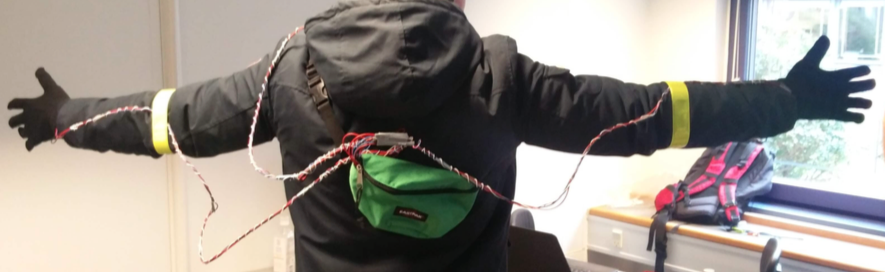
\includegraphics[width=1.01\columnwidth]{figures/enitial_prototype.png}
\caption{The early prototype used for field testing.}
\label{fig:enitial_prototype}
\end{figure} 
During the field evaluation, participants were asked to navigate to three destinations, by only utilising the vibro-tactile modality. The participants were tracked while they were navigating. The data was later used to make a heatmap, shown in figure \ref{fig:heatmap}, showing their deviation from the intended route. The predetermined route, was in a low traffic area with many bicycle paths, to ensure the safety of the participants. 
\newline
\newline 
After the field evaluation the participants were interviewed, to find out about their experience while using the system, and their thoughts regarding the vibration as a navigational tool. 
\newline
\newline  
In total five people participated in the field test. This gave sufficient amount of qualitative data. Test participants were excited about the system, they found it to be innovative and interesting due to the alternative way of navigating which enabled them to be aware of their surroundings.
%\begin{figure}
%\centering
%  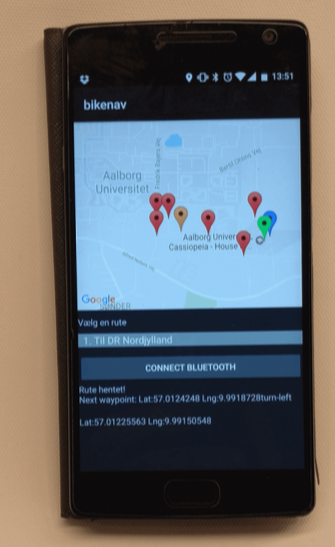
\includegraphics[width=0.6\columnwidth]{figures/first_app.png}
%  \caption{Insert a caption below each figure. Do not alter the
%    Caption style.  One-line captions should be centered; multi-line
%    should be justified. }~\label{fig:figure1}
%\end{figure}
The problems encountered in the evaluation were mostly regarding the lack of functionality in the system. Only having one navigational instruction - turn, was found to be insufficient. Test participants did not know when they arrived at their destination, which caused them to pass the intended destination, and circle around it. This is supported by the heatmap of the participants.
\begin{figure}
  \centering
  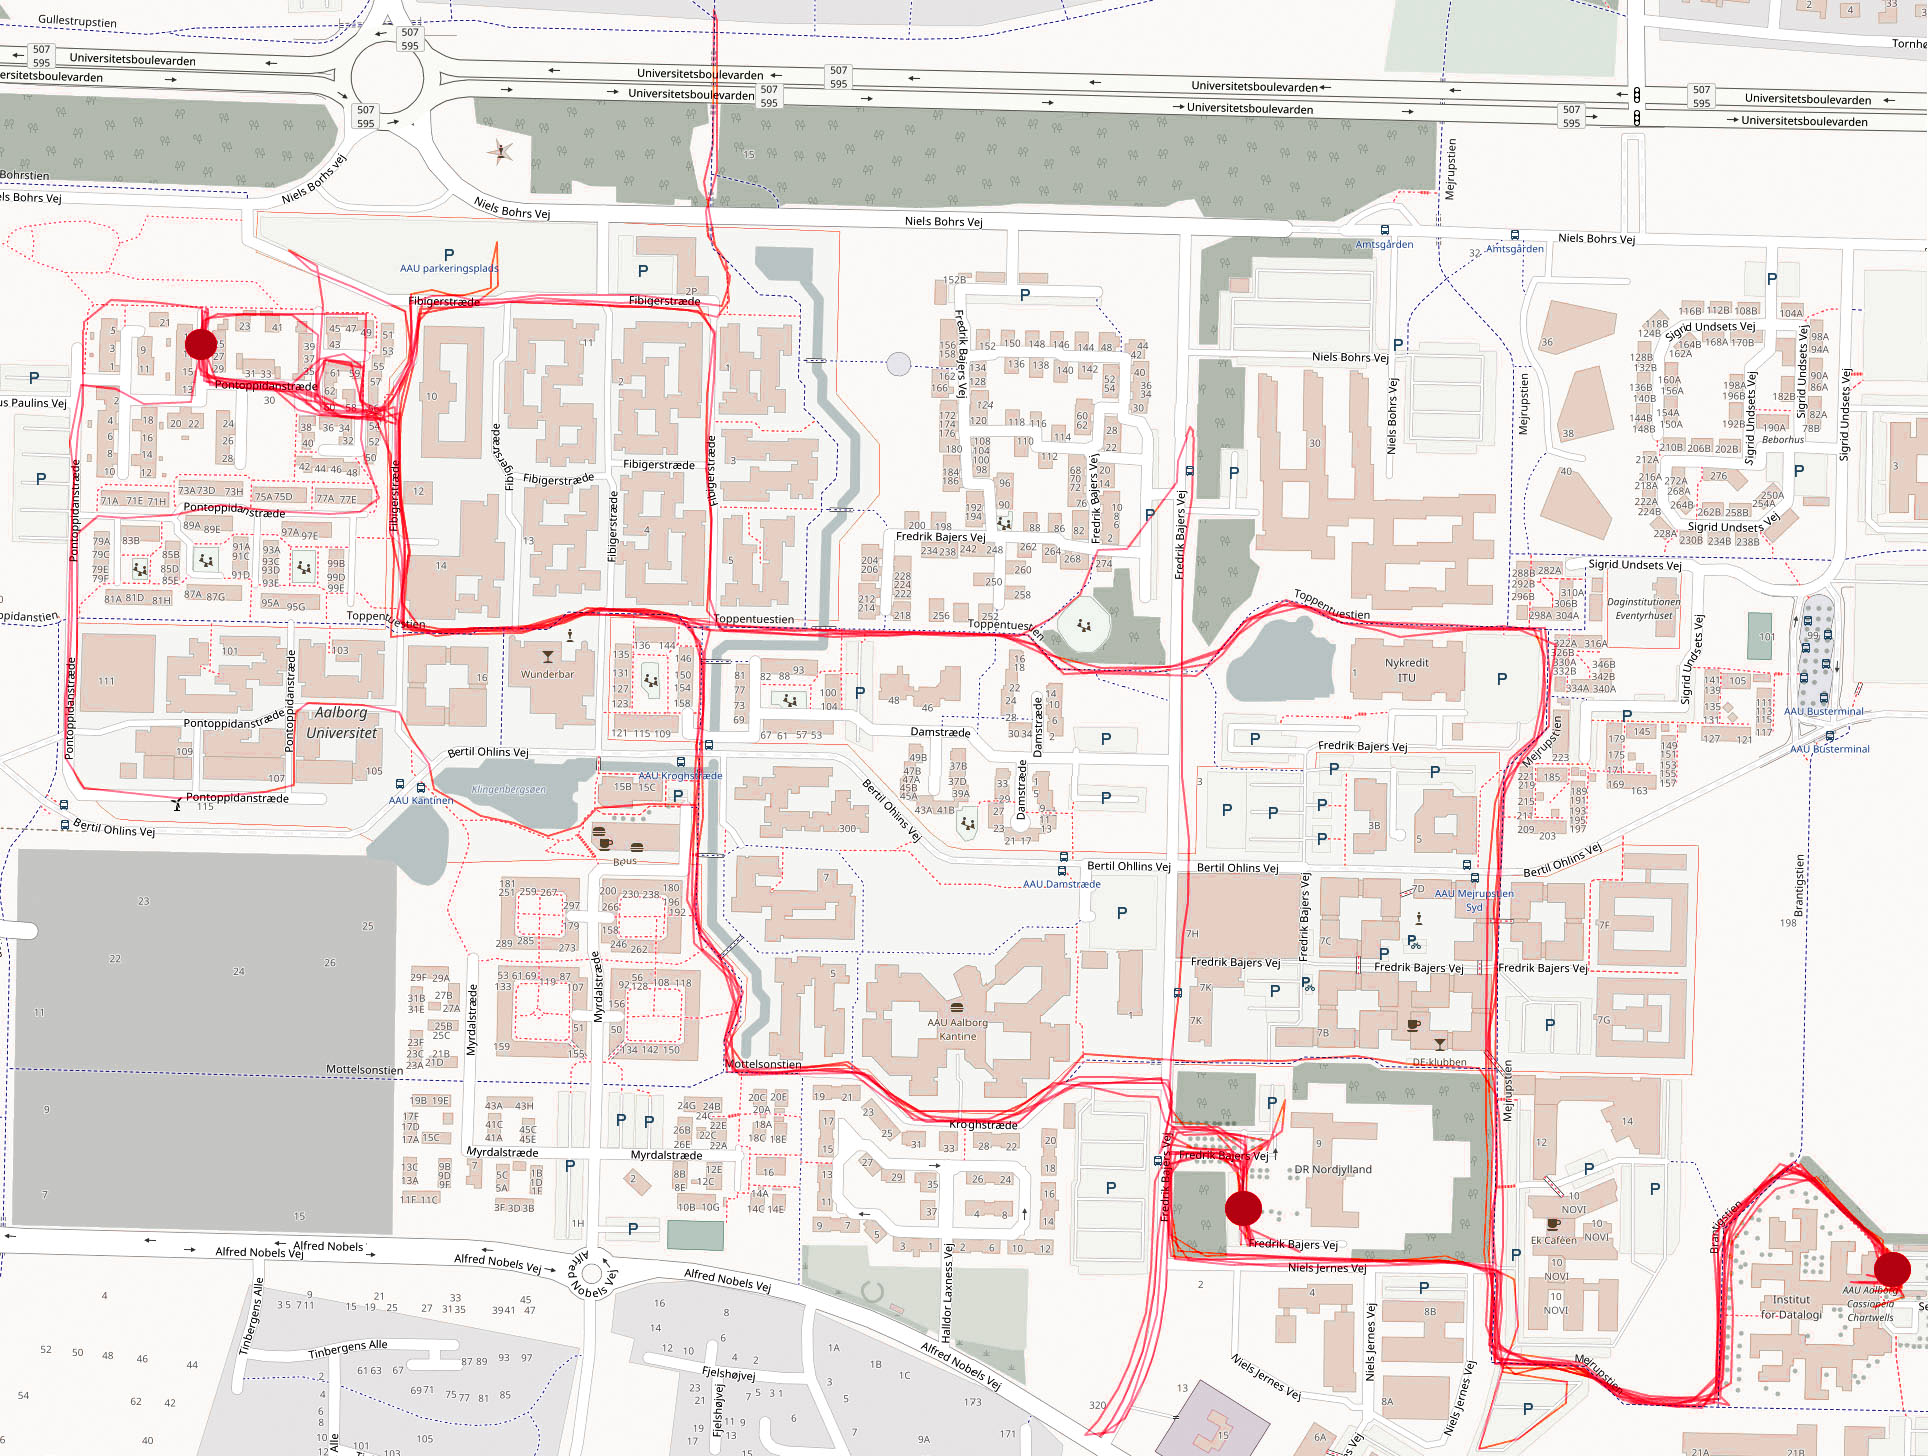
\includegraphics[width=1.02\columnwidth]{figures/heatmap.jpg}
  \caption{Tracking record of the participants' route during the first field evaluation.}
    \label{fig:heatmap}
\end{figure} 
The other problem was that participants did not know when a problem occurred. There was no feedback if the mobile phone lost connection to the wearable, this caused major problems in navigation. Additionally if a participant was cycling in a wrong direction for a long time, there was no feedback, which lead to them cycling far from the original route, in some cases the moderator had to stop the participant and inform them they were going the wrong way. This led to some participants noting that they did not know if the system was working as intended, or if they were on the right route.
\newline
\newline
Furthermore, the majority of participants thought that the system was too big, and found it to be a seasonal technology, due to the gloves. The findings from the field evaluation can be summarised to:
\begin{itemize}
\item Better information about the state of the system, to better inform the user, and keep calm.
\item Too big and seasonal technology 
\end{itemize}  
These findings lead to a new iteration, where an improved concept was developed. 
\section{Design Improvements}
After evaluating the concept in a real live scenario the system was improved on. It was found that gloves should be replaced with wristbands, making the system smaller and more aesthetically pleasing by removing connecting wires. However this change required smaller hardware components, to be able to fit inside the wristband, to keep at a size in close proximity of fitness trackers and smartwatches. The wristbands are shown in figure \ref{fig:product}.
%Physical wristbands pic
%\begin{figure}
%\centering
%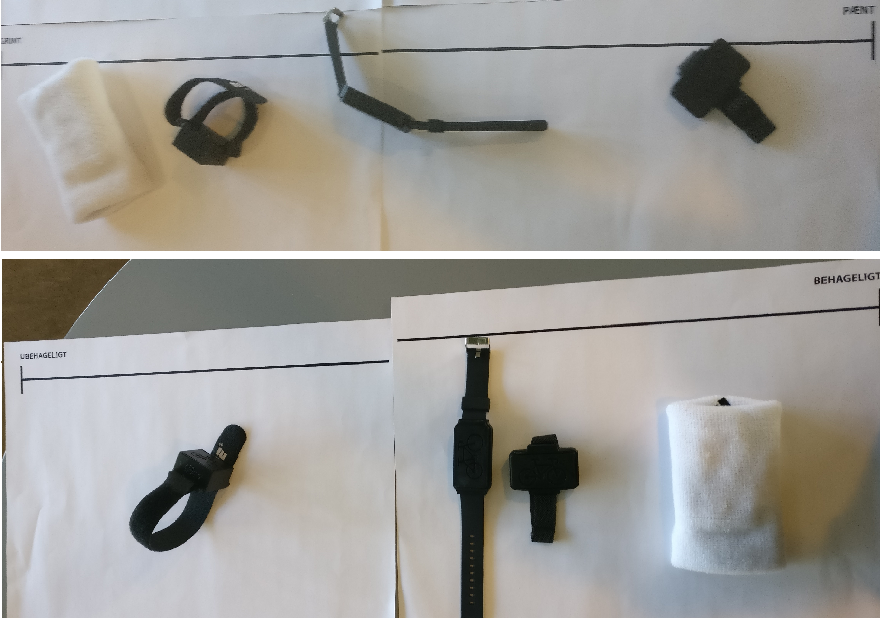
\includegraphics[width=1.02\columnwidth]{figures/wristband_evaluation.png}
%\caption{Comparison evaluation of physical wristbands}\label{fig:wristband_evaluation}
%\end{figure}
New navigation instructions were added to the system since it was found in the field evaluation that users were lacking information from the system. This lead to the system having five navigation instructions
\begin{itemize}
\item \textbf{Turn}: instructing the user to turn either left or right.
\item \textbf{U-turn}: instructing the user to turn around and go back.
\item \textbf{Arrival}: telling the user that the destination has been reached. 
\item \textbf{Problem}: telling the user that a problem with the system has arisen such as a lost connection.
\item \textbf{Heartbeat}: indicating to the user that everything is functioning as intended, and that they are on the right path.
\end{itemize} 
\begin{figure}
\centering
\includegraphics[width=1.02\columnwidth]{figures/product.png}
\caption{The developed wristbands with hardware. }\label{fig:product}
\end{figure}
A new mobile application was also developed with a cleaner interface, ability to search addresses, more detailed route visualisation and a tutorial for the system. The Tutorial informs the user of the different instructions and demonstrates the different tactons by a push buttons. This lead us to a new lab test to examine how to design the different tactons for each instruction.

\section{Second Lab Test: Designing Tactons}
When designing different tactons for each navigational instruction it was determined to design deviating tactons to find what people prefer for each of the five navigational instructions, as these have a different context. The tactons were made based on two factors that influences a tacton:
\begin{itemize}
\item \textbf{Intensity}: high and low 
\item \textbf{Rhythm}: slow and fast.
\end{itemize}
Based on these, four tactons were designed for each navigational instruction, were the tacton was described in a table designed as table \ref{tab:stage_two_tacton_design}. Each tacton differentiated in intensity and rhythm. These two parameters were chosen to be the main factors because these were the parameters used for designing tactons. The 'Spatial Location' parameter was also included in the turn instruction by only vibrating in the corresponding hand. For instructions not being side specific, vibration either alternated between hands or both hands at the same time. 
\begin{table}[!b]
\centering
\small
\begin{tabular} {p{2.0cm}p{2.0cm}p{2.0cm}}
\toprule
 & \textbf{Low intensity} & \textbf{HIGH intensity}  
\tabularnewline 
\midrule
\textbf{Slow Rhythm} & Low/Slow & HIGH/Slow  
\vspace{0.1cm} \tabularnewline
\textbf{Fast Rhythm} & Low/Fast & HIGH/Fast 
\vspace{0.1cm} 
\tabularnewline
\bottomrule
\end{tabular}
\caption{The four way differentiation between tactons.}
\label{tab:stage_two_tacton_design}
\end{table}
\noindent
\newline
\newline
19 participants were included for this test. Each tactons were sent to the test participant three times, and afterwards the participant had to evaluate the tacton on \textit{suitability}; based on the context of navigational instruction, and \textit{preference}; whether they liked it. This procedure was repeated till all 20 (four for each navigational instruction) tactons were evaluated.
\newline
\newline
This lab test showed that instructions that required immediate attention (Arrival, Problem), had to be HIGH/FAST or HIGH/SLOW, indicating that high intensity is important parameter when there is a need for attention. 
While navigational instructions that should stay in users periphery or inform users gradually (Heartbeat, U-turn and Turn) low intensity and slow rhythm was sufficient. This information was used when choosing the tactons that were implemented in the physical system.  
\section{Second Field test}
The final field evaluation was performed in the same settings as the first field test. The users were handed the system and had to  find out how to use it themselves, with help from the tutorial in the mobile application. When they were familiar with the system - the evaluation began. The same route was chosen as in the first field test with the same three destinations, making it possible to compare between the earlier prototype. 
\newline
\newline
The participants were given one destination at a time and had to use the system to navigate to the location. After the field evaluation, an interview was conducted with question based on the Calm Technology principles. This was done to evaluate the ''calm'' quality of the system. In total nine people participated in the evaluation.
\begin{figure}[!b]
  \centering
  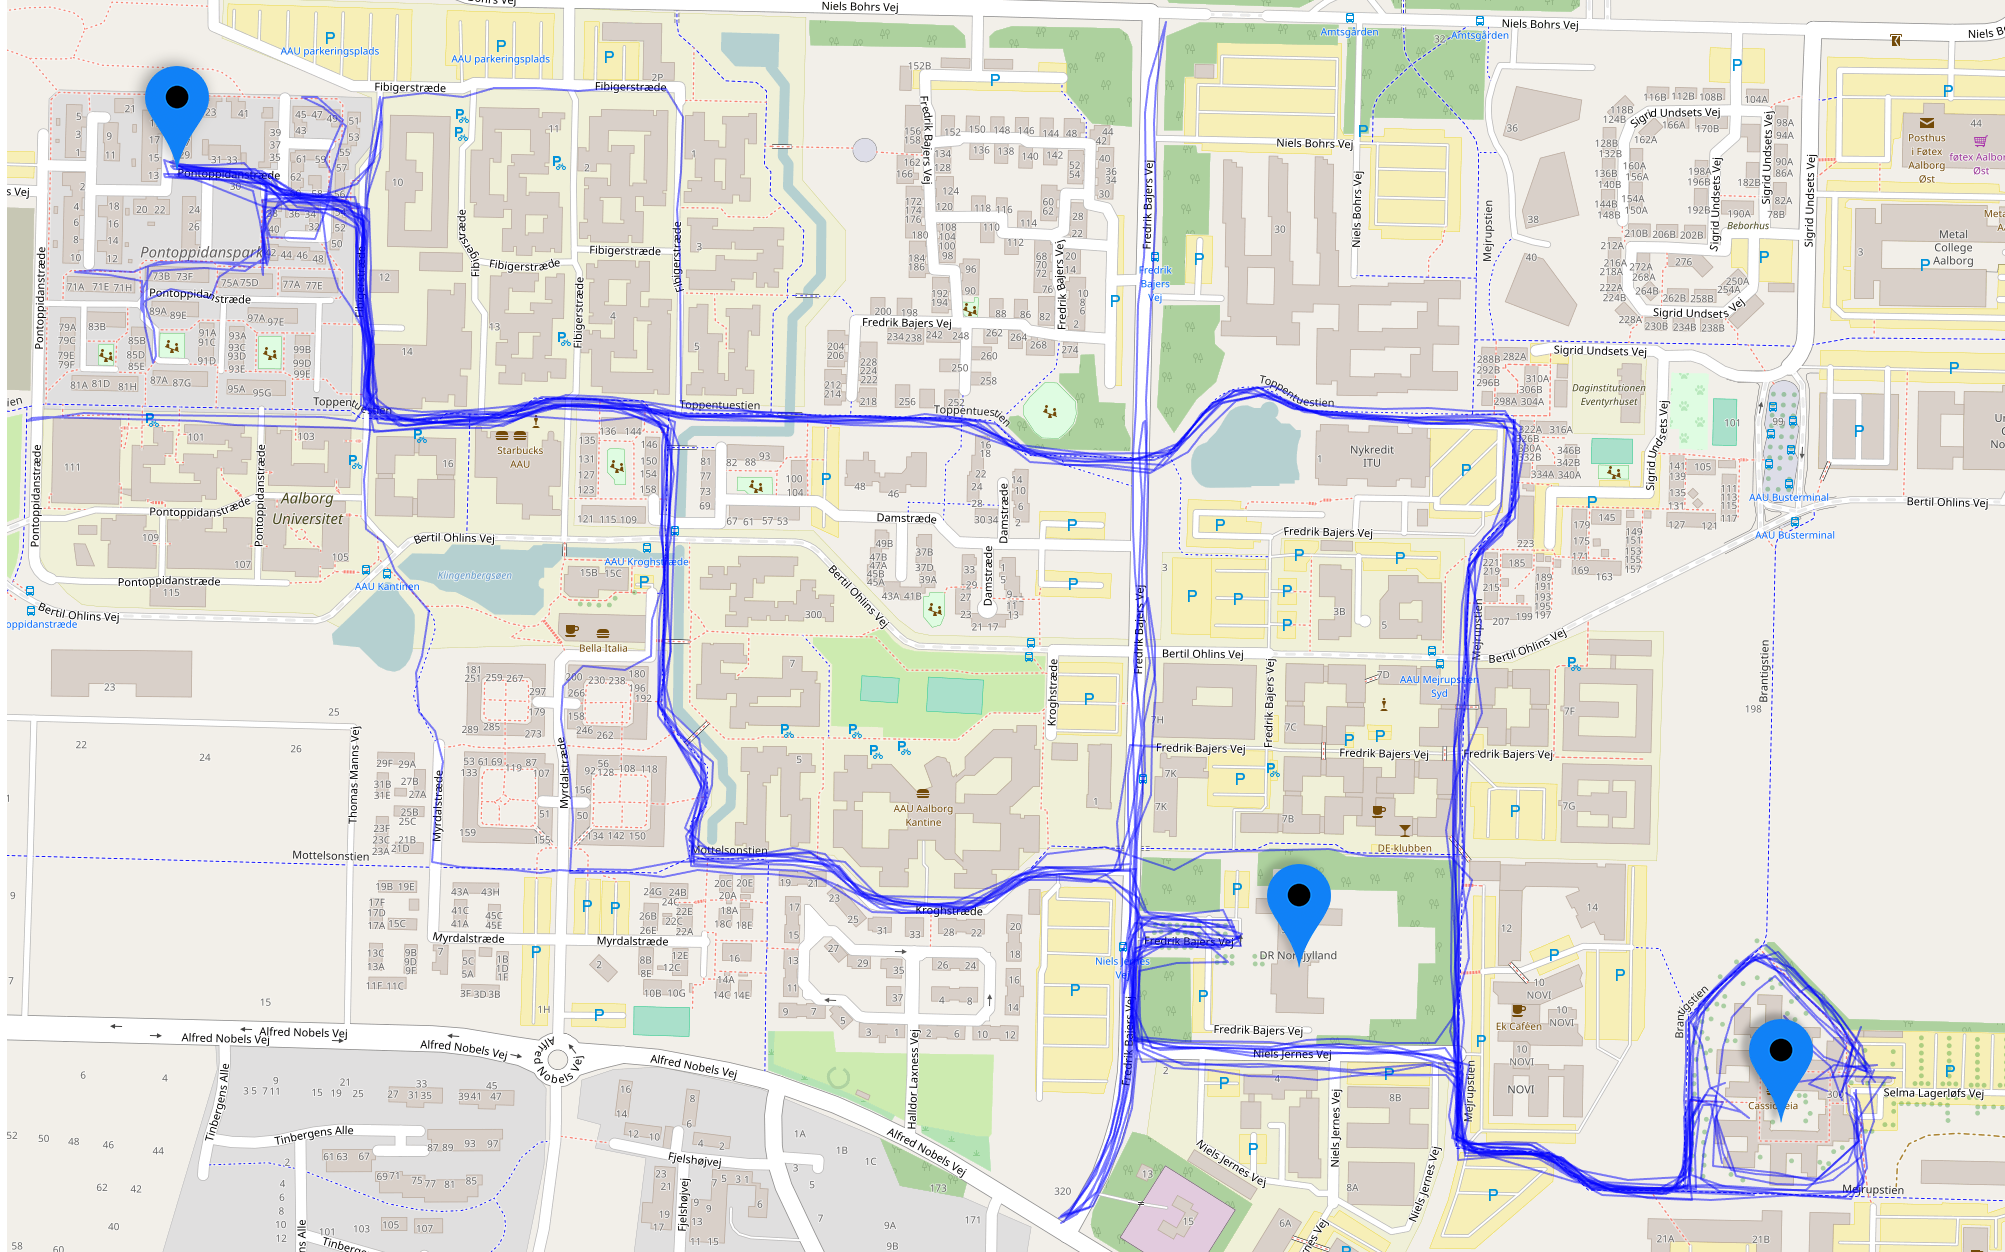
\includegraphics[width=1.02\columnwidth]{figures/stort_heat_map.png}
  \caption{The tracking of the nine participants' routes for the second field evaluation.}
  \label{fig:stort_heat_map}
\end{figure}
\section{Results}
In the evaluation it was found that the system performed well, and many test participants expressed that the system required less attention than traditional navigational systems, such as Google maps and GPS. 
\newline
\newline
Additionally, the participants trusted the system, even though some issues occurred during the navigation. The Heartbeat instruction was originally designed to assure the user that the system is functioning correctly. But the evaluation proved the opposite, with participants explaining that the heartbeat was confusing and obtrusive to them. This was due to the fact that they were expecting instructions, and the heartbeat was also perceived as an instruction requiring to an activity in response, when actuality, it was only meant as assurance that every is connected and working as intended.
\newline
Another issue was with the turn instruction. The turn instruction works by starting at a waypoint when approaching a turn, based on speed and distance. When two turns was too close to each other, the tacton for the second turn would be started before the user had performed the first turn. This made them miss turns.
\newline
\newline 
However, even though they cycled in the wrong direction after missing a turn or due to other problems, no help was required from the test monitor to find the right way again, in contrary to the first field evaluation. Here the mobile application was usually used to see the route or to connect to the wearables again. 
\newline
Based on the interview, the majority of the calm technology principles were met in the system. 

\section{Conclusion}
Vibration worked well as an alternative way of sending navigational instructions. It was found to be unobtrusive, when only giving the relevant information, as required by Calm Technology principles. 
And even though it is important to inform and keep calm, the information should be considered carefully, since too much information can do the opposite and cause confusion. This was the case in the second field evaluation, where heartbeat confused the participants. When designing tactons, it is important to make them clearly distinguishable, and it should be avoided to rely on the users ability to easily distinguish many different tactons. However it should be noted that some related work suggests that users can be trained to better distinguish tactons. 
\newline
The system is still too big for some test participants, and therefore developing an even smaller wearable, not using prototype hardware components as Arduino, would be optimal. 

\section{Acknowledgements}
We would like to extend our sincerest gratitude to Dimitrios Raptis for his help with this paper. We would also like to thank all of our participating subjects for their help in these studies. Finally we would like to give thanks to our study secretary Lone Elgaard.
% Balancing columns in a ref list is a bit of a pain because you
% either use a hack like flushend or balance, or manually insert
% a column break.  http://www.tex.ac.uk/cgi-bin/texfaq2html?label=balance
% multicols doesn't work because we're already in two-column mode,
% and flushend isn't awesome, so I choose balance.  See this
% for more info: http://cs.brown.edu/system/software/latex/doc/balance.pdf
%
% Note that in a perfect world balance wants to be in the first
% column of the last page.
%
% If balance doesn't work for you, you can remove that and
% hard-code a column break into the bbl file right before you
% submit:
%
% http://stackoverflow.com/questions/2149854/how-to-manually-equalize-columns-
% in-an-ieee-paper-if-using-bibtex
%
% Or, just remove \balance and give up on balancing the last page.
%
\balance{}

% REFERENCES FORMAT
% References must be the same font size as other body text.
\bibliographystyle{SIGCHI-Reference-Format}
\bibliography{sample}

\end{document}

%%% Local Variables:
%%% mode: latex
%%% TeX-master: t
%%% End:
